\begin{figure}[ht!]
	\captionsetup[subfigure]{justification=centering}
	\centering
	\begin{subfigure}[t]{0.5\linewidth}
		\centering
		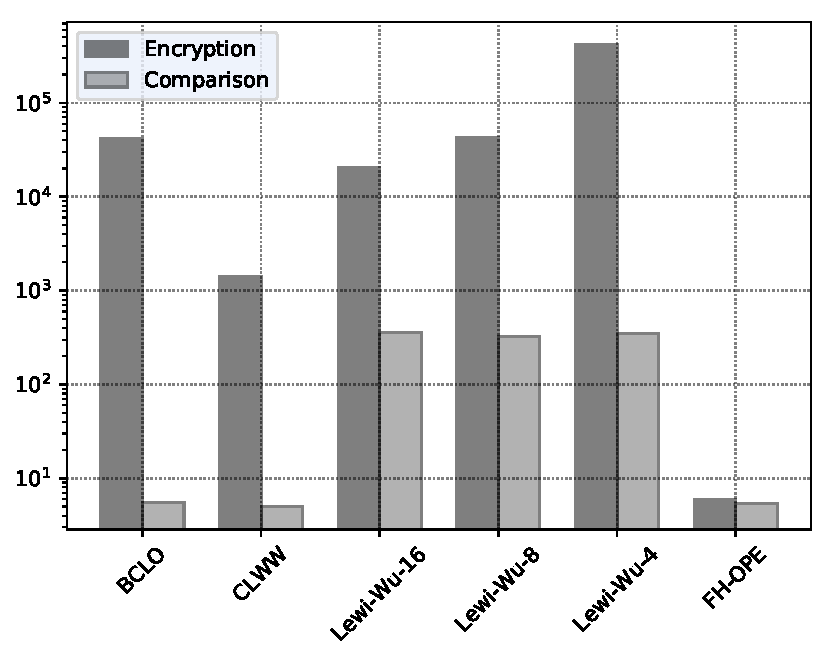
\includegraphics[height=97pt,width=\linewidth]{schemes-benchmark.pdf}
		\setlength{\abovecaptionskip}{-5pt}
		\setlength{\belowcaptionskip}{-5pt}
		\caption{Schemes benchmark (time in microseconds, log scale). Lewi-Wu parameter is the number of blocks.}
	\end{subfigure}%
	~ % chktex 39
	\begin{subfigure}[t]{0.5\linewidth}
		\centering
		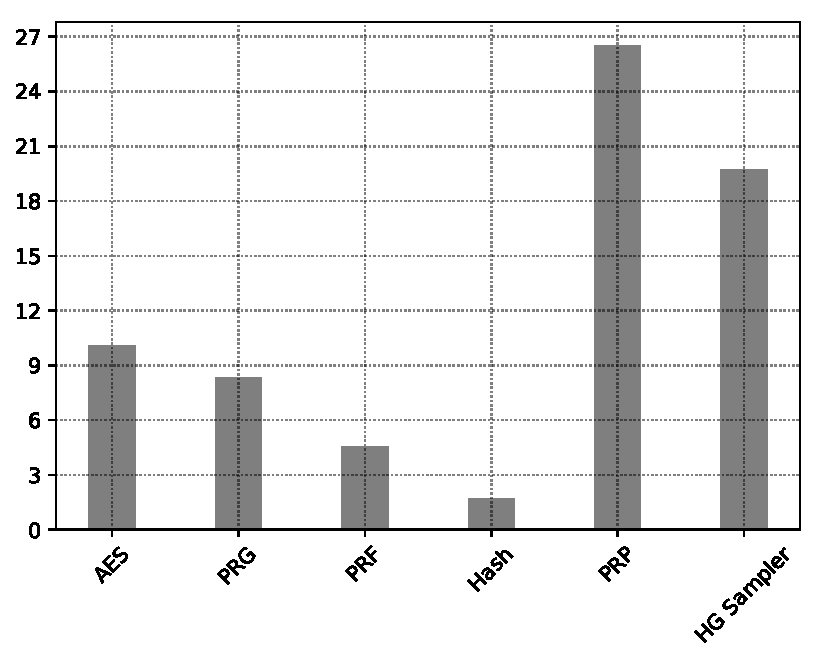
\includegraphics[height=97pt,width=\linewidth]{primitives-benchmark.pdf}
		\setlength{\abovecaptionskip}{-5pt}
		\setlength{\belowcaptionskip}{-5pt}
		\caption{Primitives benchmark (time in microseconds)}
	\end{subfigure}%
	\caption{Benchmarks of the schemes and primitives}\label{fig:benchmarks}
\end{figure}

% schemes benchmark data /benchmark/2018-09-28_00-37-08/
% primitives benchmark data /primitives/2018-09-27_20-04-01/
